Funksjonen $\vec{F}: \mathbb{R}^2 \to \mathbb{R}^2$
skal speile alle punkter om linjen $y = 1 - x$.\\
Finn $A$ og $\vec{c}$ s.a. $\vec{F}$ kan skrives som
$\vec{F}(x,y) = A\vec{x} + \vec{c}$.\\\\
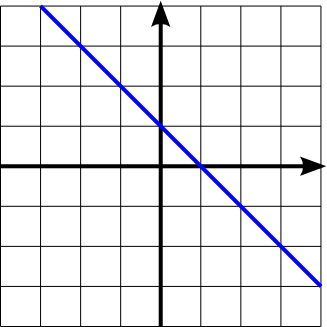
\includegraphics[width=0.5\textwidth]{./mat1110-oblig1-oppg1.png}

\paragraph{Finne $\vec{c}$ vektor} \mbox{} \\
Jeg tester punktet $(0,0)$ for å gjøre det enklere for meg selv.\\
Man kan se grafisk at
$\vec{F}(0,0) = (1,1)$.\\
Det vil si at
$$\vec{F}(0,0) = A\colvec{0}{0}+\vec{c}
= \colvec{0}{0}+\vec{c} = \vec{c} = (1,1)$$
Dermed er $\vec{c}$ funnet.

\paragraph{Finne matrisen A (Del 1)} \mbox{} \\
Tester tilfeldige punkter og ser hva svaret skal bli.\\
Man ser grafisk at
$\vec{F}(-4,1) = (0,5)$.\\
Siden $A$ er ukjent, definerer jeg den som
$\left( \begin{matrix}
  x & y \\
  z & u
\end{matrix} \right)$
Det vil si at
$$\vec{F}(-4,1) = A\colvec{-4}{1}+\vec{c}
= \colvec{-4x+y}{-4z+u} + \colvec{1}{1} = (0,5)$$
Dette gir
$$-4x + y + 1 = 0 $$
$$-4z + u + 1 = 5$$
$$y = 4x - 1$$
$$u = 4z + 4$$

\paragraph{Finne matrisen A (Del 2)} \mbox{} \\
Tester enda et tilfeldig punkt.\\
$\vec{F}(1,0) = (1,0)$.\\
Så spennende at dette punktet ikke flyttes.\\
$$\vec{F}(1,0) = A\colvec{1}{0} + \vec{c}
= \colvec{x}{z} + \colvec{1}{1}$$
Dette gir
$$x+1=1$$
$$z+1=0$$
$$x = 0$$
$$z = -1$$
Satt inn i ligningene fra Del 1
$$y = 4x-1 = 0-1$$
$$y = -1$$
$$u = 4z+4 = -4+4$$
$$u = 0$$

\paragraph{Resultat}
Nå er A funnet
$$
A =
\left( \begin{matrix}
  x & y \\
  z & u
\end{matrix} \right) =
\left( \begin{matrix}
  0 & -1 \\
  -1 & 0 
\end{matrix} \right)
$$
...og $\vec{c}$ hadde vi fra før
$$\vec{c} = \colvec{1}{1}$$
